\documentclass[helvetica, 10pt]{article}

% If you're new to LaTeX, here's some short tutorials:
% https://www.overleaf.com/learn/latex/Learn_LaTeX_in_30_minutes
% https://en.wikibooks.org/wiki/LaTeX/Basics

% Formatting
\usepackage{blindtext}
\usepackage[T1]{fontenc}
\usepackage[utf8]{inputenc}
\usepackage[margin=1in]{geometry}

% Math
% https://www.overleaf.com/learn/latex/Mathematical_expressions
\usepackage{amsmath, amsfonts, amssymb, mathtools}

% Images
% https://www.overleaf.com/learn/latex/Inserting_Images
\usepackage{graphicx, float}

% Algorithms
% https://www.overleaf.com/learn/latex/algorithms
% https://en.wikibooks.org/wiki/LaTeX/Algorithms
\usepackage[ruled,vlined]{algorithm2e}
\usepackage{algorithmic}

% Code syntax highlighting
% https://www.overleaf.com/learn/latex/Code_Highlighting_with_minted
\usepackage{minted}
\usemintedstyle{borland}


% ====================== TITLE =========================================
\title{Artificial intelligence - Project 1 \\ - Search problems - }

% introduceti numele autorului aici
\author{Birlutiu Claudiu-Andrei}
\date{29/10/2021}

\begin{document}

\maketitle
\thispagestyle{empty}

% ====================== UNINFORMED SEARCH =============================
\section{Uninformed search}

% ============================================= DFS ============================================= 
\subsection{Question 1 - Depth-first search}
% enuntul intrebarii
In aceasta sectiune va fi prezentatata implementarea problemei 2.14 din laborator, al carei enunt este: \newline


\textit{"In search.py, implement \textbf{Depth-First search(DFS) algorithm} in  function \textit{depthFirstSearch}. Don’t  forget that DFS graph search is graph-search with the frontier as a LIFO queue(Stack)."}.


\subsubsection{Code implementation}
In continuare se regaseste codul propus pentru implemetarea acestui \textbf{algoritm de cuatare}. In incercarea de implementare si apoi testare a solutiei propuse am apelat mai multe comenzi din terminal pentru a vedea evolutia agentului \textit{pacman} in procesul de cautare a solutiei sale.   \newline\newline\newline    \\

\textbf{Code:}
% a se completa fisierul code/dfs.py
\inputminted[linenos]{python}{code/01_dfs.py}

\textbf{Explanation:}
\begin{itemize}
    \setlength\itemsep{0em}
    \item  la linia 4 am importat structura de date Stack implementata in achetul util; aceasta structura permite adaugarea unui element, scoaterea elementului cel mai recent adaugat si permite verificarea starii acesteia ( daca stiva e goala)
    \item  la linia 4 ne declaram o variabila de tipul Stack, in care se vor adauga nodurile din frontiera in momentul expandarii grafului de cautare
    \item  la linia 6 ne declaram o lista ce va contine nodurile deja explorate
    \item  la lina 7 ne declaram nodul de start; Pentru aceasta s-a crea o clasa ce reprezinta structura de date a unui nod. Atributele acestei clase sunt: starea (pozitia din grid), nodul parinte, action (actiunea prin care s-a ajuns la el) si costul total al caii de la radacina 
    \item la linia 8 se adauga in frontiera nodul de start, iar apoi se intra in bucla while a carei conditii de terminare il reprezinta testul pe frontiera. In cazul in care nu va mai exista nciun nod in frontiera va arata ca nu mai este niciun nod care sa fie expandat
    \item incepand cu linia 11 pana la linia 24 se va descrie ideea algorimului dfs; intotdeauna se va lua nodul cel mai recent adaugat in frontiera: daca acesta este scopul problemei de cautare, atunci algorimul se va opri si va returna solutia, iar in caz contrar va continua prin expandarea succesorilor acestui nod si adaugarea lor in frontiera daca nu au fost deja adaugati. Deoarece avem acest test de verificare a nodurilor (daca sunt in lista de noduri explorate) inainte de a fi adaugate in frontiera, va determina o parcurgere de tip \textbf{graph search}
    \item la linia 14 se verifica daca nodul extras din frontiera a fost deja explorat, in caz afirmativ va fi ignorat. Teoretic acest nod a fost adaugat de mai multe ori in frontiera deaorece nu s-a putut face testul de apartenenta pe structura Stack
    \item pentru reconstructia actiunilor prin care s-a ajuns la nodul scop din nodul start s-a implementat functia \textbf{construct\_path(node)}, functie ce reconstruieste calea pe baza relatiei copil parinte
    \item valoarea returnata de functie va fi o lista cu actiunile ce urmeaza sa le execute agentul din pozitia initiala pana la scop

\end{itemize}


\textbf{Commands:}
\begin{itemize}
    \setlength\itemsep{0em}
    \item  -l tinyMaze -p SearchAgent -a fn=dfs 
    \item  -l bigMaze -z .5 -p  SearchAgent -a fn=dfs 
    \item  -l mediumMaze -p -z .5  SearchAgent -a fn=dfs
        
\end{itemize}

\subsubsection{Questions}



\textbf{Q1:} Is the found solution optimal? Explain your answer.


\textbf{A1:} Nu gaseste solutia optima, deoarece algorimul nu tine seama de costul drumului pe care il alege. Cum ii zice si numele, el va cauta cat mai mult in adancime, astfel va ajunge sa exploreze o ramura pana la nivelul cel mai de jos si apoi daca nu va reusi sa gaseasca solutia va cauta si pe celelalte ramuri  la un nivel mai apropiat de radacina si unde s-ar putea sa fie solutia \newline


\textbf{Q2:} Run\textit{ autograder python autograder.py} and write the points for Question 1.


\textbf{A2:} Question q1: 4/4


\subsubsection{Personal observations and notes}
Pentru bigMaze costul total al caii este de 210, iar numarul de noduri explorate este de 390.Pentru mediumMaze costul total al caii este de 130, iar numarul de noduri explorate este de 146.Se vor face niste comparatii cu celelalte rezultate obtinute pentru ceilalti algoritmi implementati la fiecare subsectiune. 
\vspace{0.75cm}

% ============================================= BFS ============================================= 
\subsection{Question 2 - Breadth-first search}
% enuntul intrebarii
In continuare va fi descris exercitiul 2.15 din laborator:\newline


\textit{"In \textbf{search.py}, implement the \textbf{Breadth-First search} algorithm in function \textit{breadthFirstSearch}."}.


\subsubsection{Code implementation}
In continuare se regaseste codul propus pentru implemetarea acestui \textbf{algoritm de cuatare}. In incercarea de implementare si apoi testare a solutiei propuse am apelat mai multe comenzi din terminal pentru a vedea evolutia agentului \textit{pacman} in procesul de cautare a solutiei sale.   \newline    \\


\textbf{Code:}
% a se completa fisierul code/bfs.py
\inputminted[linenos]{python}{code/02_bfs.py}


\textbf{Explanation:}
\begin{itemize}
    \setlength\itemsep{0em}
    \item la linia 5 se importa structura de date Queue implementatata in util; ceasta structura permite adaugarea unui element, scoaterea elementului cel mai vechi adaugat si permite verificarea starii acesteia (daca e goala sau nu)
    \item la linia 8 se declara o lista vida in care se vor adauga nodurile explorate 
    \item in cazul acestei solutii va fi nevoie de o coada pentru a descrie frontiera 
    \item la liniile 12 si 13 va fi creat nodul de start (care are aceeasi structura descrisa la cerinta anterioara) si va fi adaugat in frontiera
    \item ideea acestui algoritm consta in scoaterea nodurilor din frontiera in ordinea in care au fost aduagate si expandarea acestora prin determinarea succesorilor si adaugarea lor in frontiera. Deoarece si in acest caz se merge pe o abordare de tip \textbf{graph search}, ianinte de a adauga in fronitera un nod se va verifica daca acesta nu a fost explorat deja.
    \item deoarece si in cazul cozii implementate in util nu putem sa determinam daca un element e deja in coada, am mers pe aceeasi idee de a adauga duplicate, iar cand se vor extrage se vor ignora - la linia 19 e tratat acest caz
    \item in cazul in care se ajunge la nodul scop se va opri cautarea si se va returna solutia problemei
    \item pentru a construi calea de la nodul de start la nodul scop cu actiunile necesare se va apela functia \textbf{construct\_path(node)}

\end{itemize}


\textbf{Commands:}
\begin{itemize}
    \setlength\itemsep{0em}
    \item  -l bigMaze -z .5 -p  SearchAgent -a fn=bfs
    \item  -l mediumMaze -z .5 -p  SearchAgent -a fn=bfs
    \item  -l tinyMaze -z .5 -p  SearchAgent -a fn=bfs
        
\end{itemize}

\subsubsection{Questions}
This sub-section is dedicated to the additional questions that come along with the exercise. Please answer to the following questions:\newline


\textbf{Q1:} Is the found solution optimal? Explain your answer. 


\textbf{A1:} Da, bfs va gasi intotdeuana solutia optima daca costul tranzitiilor este acelasi. In cazul lui pacman costul este de 1 pentru orice tranzitie dintr-o stare in alta. De fapt, bfs va gasi calea cea mai scurta pana la nodul scop, deoarece el parcurge graful nivel cu nivel. Cu alte cuvinte, cand se va explora un nod de la un nivel, toate nodurile din nivelele mai apropoiate de radacina au fost explorate. 


\textbf{Q2:} Run autograder \textit{python autograder.py} and write the points for Question 2.


\textbf{A2:} Question q2: 4/4


\subsubsection{Personal observations and notes}
Pentru bigMaze costul total al caii este de 210, iar numarul de noduri explorate este de 620.Pentru mediumMaze costul total al caii este de 68, iar numarul de noduri explorate este de 269. Diferentele ce se observa intre dfs si bfs sunt la nivelul nodurilor explorate si la costul caii gasite. Observam ca bfs gaseste mereu calea optima, dar va explora mult mai multe noduri decat o face dfs.

\vspace{0.75cm}



\subsection{References}
R. Stuart, N. Peter, Artificial Intelligence: A Modern Approach, 4th US ed., capitol 3, [online]

% ====================== INFORMED SEARCH ===============================
\section{Informed search}
\graphicspath{{images/}}
% ============================================= A*  ============================================= 
\subsection{Question 4 - A* search  algorithm}
% enuntul intrebarii
In sectiunea urmatoare va fi descris exercitiul 3.2 din laborator \newline


\textit{"Go to aStarSearch in search.py and implement \textbf{A* search algorithm}. A* is graphs search with the frontier as a priorityQueue, where the priority is given bythe function g=f+h"}.


\subsubsection{Code implementation}
In continuare se regaseste codul propus pentru implemetarea acestui algoritm de cuatare. In incercarea de implementare si apoi testare a solutiei propuse s-au apelat mai multe comenzi din terminal pentru a vedea evolutia agentului pacman in procesul de cautare a solutiei sale \\

\textbf{Code:}
% a se completa fisierul code/4_a_star.py
\begin{listing}[h]
    \inputminted[linenos]{python}{code/04_a_star.py}
    \caption{Solution for the A* algorithm.}
    \label{listing:a_star}
\end{listing}


\textbf{Explanation:}
\begin{itemize}
    \setlength\itemsep{0em}
    \item in cadrul acestui algoritm este nevoie de o structura de date speciala pentru frontiera. Aceasta structura va fi PriorityQueue, iar prioritatea nodurilor ce se vor afla in frontiera va fi data de costul drumului pana in acel nod si de estimarea costului pana la scop(determinata prin intermediul unei euristici). La linia 11 este creata o astfel de structura pe care o gasim implementata in util
    \item pentru nod-uri s-a folosit aceeasi structura folosita si in cadrul solutiei pentru dfs si bfs
    \item ideea acestui algoritm este de a alege din frontiera nodul cel mai bun ca si candidat pentru solutia optima, nod ce va fi testat daca e scop si in caz afirmativ se va returna solutia sau in caz contrar ii vor expandati succesorii si adaugati in frontiera daca nu au fost expandati inainte. 
    \item linia 29 este esentiala in cadrul acestei solutii, deoarece daca pentru un nod se gaseste un copil ce se afla in frontiera, prioritatea acetuia se va modifica daca functia de evaluare a costului in aceasta conjuctura e mai mica decat cea de dinainte. Aceasta va determina intotdeuana o solutie optima a algoritmului. 
    \item pentru a construi calea de la nodul de start la nodul scop cu actiunile necesare se va apela functia \textbf{construct\_path(node)}

\end{itemize}


\textbf{Commands:}
\begin{itemize}
    \setlength\itemsep{0em}
    \item  -l bigMaze -z .5 -p SearchAgent -a fn=astar,heuristic=manhattanHeuristic
    \item  -l mediumMaze -z .5 -p SearchAgent -a fn=astar,heuristic=manhattanHeuristic
        
\end{itemize}

\subsubsection{Questions}
This sub-section is dedicated to the additional questions that come along with the exercise. Please answer to the following questions:\newline


\textbf{Q1:} Does A* and UCS find the same solution or they are different?


\textbf{A1:} Depinde de euristica folosita pentru estimarea costului pana la nodul scop. Daca euristica este constana 0, atunci A* star este identinc cu UCS, iar daca euristica e buna (admisibila si consistenta) A* ar trebui sa ofere aceeasi solutie ca UCS, solutie care e si optima de altfel.


\textbf{Q2:} Does A* finds the solution with fewer expanded nodes than UCS?


\textbf{A2:} Cu cat euristica se apropie de adevar, cu atat algoritmul va expanda mai putine noduri, deaorece el se va duce pe o abordare de tip Greedy. Deoarece A* are in logica sa si o abordare de tip Greedy, el va expanda mai putine noduri decat UCS.

\textbf{Q3:} Run autograder \textit{python autograder.py} and write the points for Question 4 (min 3 points).


\textbf{A3:} Question q3: 4/4


\subsubsection{Personal observations and notes}
Pentru bigMaze costul total al caii este de 210, iar numarul de noduri explorate este de 549.Pentru medium-Maze costul total al caii este de 68, iar numarul de noduri explorate este de 221.S-a folosit pentru aceste teste euritstica \textit{manhattan} Observam ca avem solutia optima pentru cele doua probleme, iar numarul de noduri expandate este mai putin decat la bfs.
\vspace{0.75cm}

% ============================================= All Corners ===================================== 
\subsection{Question 5 - Find all corners - problem implementation}
% enuntul intrebarii
In urmatoare subsectiune va fi prezentat exercitiul 3.3 din laborator al carui enunt e: \newline


\textit{"Pacman  needs  to  find  the  shortest  path  to  visit  all  the  corners,regardless  there  is  food  dot  there  or  not. Go to \textbf{CornersProblem} in searchAgents.py and propose a representation of the state of this search problem. It might help to look at the existing implementation for PositionSearchProblem. The representation should include only the information necessary to reach the goal. Read carefully the comments inside the class CornersProblem."}.


\subsubsection{Code implementation}
In continuare se regaseste codul propus pentru implemetarea acestei clase ce descrie o noua problema. In incercarea de implementare si apoi testare a solutiei propuse s-au apelat mai multe comenzi din terminal pentru a vedea evolutia agentului pacman in procesul de cautare a solutiei sale \\

\textbf{Code:}

% a se completa fisierul code/corner_problem.py
\inputminted[linenos]{python}{code/05_corner_problem.py}


\textbf{Explanation:}
\begin{itemize}
    \setlength\itemsep{0em}
    \item  la linia 24 este declarat un atribut al \textit{problemei} ce se refera la starea colturilor. Va fi declarat un dictionar de forma \textbf{colt:vizitat?}- unde prin \textit{vizitat?} se intelege o valoare buleana (True sau False). Acest dictionar va contine informatia despre toate colturile.
    \item la liniile 30 -32 se verifica pentru fiecare colt daca e pozitia de start sau in acel loc e un zid si in caz afirmativ il vom marca vzitat in dictionarul atribut
    \item la linia 37 se va lua o tupla pentru pozitia de start, care va contine pozitia in grid si dictionarul cu informatia despre colturi
    \item metoda \textbf{getStartState} va returna tupla formata din starea initiala si starea colturilor la momentul initial
    \item scopul problemei de fata este de a vizita toate colturile. Se ajunge la scop in momentul in care toate valorile din dictionar sunt true. Metoda \textbf{isGoalstate(self,state)} va fi implementata printr-o simpla parcurgere a valorilor din dictionar si daca se intalneste o valoare de False va returna False, iar daca nu, va returna True
    \item liniile 58-79: metoda \textbf{expand} este similara cu cea de la \textit{PositionSearchProblem} 
    \item liniile 105-122 ceea ce lipseste in metoda \textbf{getnextState} este determinarea noului dictionar al colturilor asociat starii.
\end{itemize}

\textbf{Commands:}
\begin{itemize}
    \setlength\itemsep{0em}
    \item  -l mediumCorners -p SearchAgent -a fn=bfs,prob=CornersProblem
    \item  -l mediumCorners -p SearchAgent -a fn=astar,heuristic=cornersHeuristic,prob=CornersProblem
    \item   -l mediumCorners -p SearchAgent -a fn=astar,prob=CornersProblem
\end{itemize}
\subsubsection{Questions}

\textbf{Q1:} For mediumCorners, BFS expands a big number - around 2000 search nodes.  It’s time to see that A* with an admissible heuristic is able to reduce this number. Please provide your results on this matter. (Number of searched nodes).

\textbf{A1:} Bfs: 1966 noduri expandate; O euristica admisibila pentru aceasta problema poate fi nullEuristic. Pentru aceasta euristica numarul de noduri expandate a ramas 1966. Pentru cazul in care am apelat cu o eurirstica consistenta si admisibila (cornersHeuristic -implementatata in sectiunea urmatoare), numarul s-a redus la 783 de noduri expandate.


\subsubsection{Personal observations and notes}
Initial am creat o clasa \textbf{CornerState} care imi descria structura pentru o stare din aceasta problema apoi am vazut ca se doreste folosirea unei tuple, deoarece cand se prelua pozitia se dorea indexarea (state[0] -linia 85) 
\vspace{0.75cm}

% ============================================= Consistent heuristic ============================= 
\subsection{Question 6 - Find all corners - Heuristic definition}
% enuntul intrebarii
In sectiunea aceasta este explicat si rezolvat exercitiul 3.4 din laborator:  \newline


\textit{"Implement  a  consistent  heuristic  for  CornersProblem. Go to the function \textbf{cornersHeuristic} in searchAgent.py."}.


\subsubsection{Code implementation}
 In continuare se regaseste codul propus pentru implemetarea acestei metode ce descrie o euristica consistenta pentru problema CornersProblem. In incercarea de implementare si apoi testare a solutiei propuse s-au apelat mai multe comenzi din terminal pentru a vedea evolutia agentului pacman in procesul de cautare a solutiei sale \newline\newline\\


\textbf{Code:}

% a se completa fisierul code/6_consisntency_heuristic.py
\inputminted[linenos]{python}{code/06_consistent_heuristic.py}


\textbf{Explanation:}
\begin{itemize}
    \setlength\itemsep{0em}
    \item pentru ca o euristica sa fie consistenta si admisibila ea trbuie sa indeplineasca niste conditii:\newline
    \textbf{admisibilitate}: h(n) <= h*(n) , unde h* este costul real pana la cel mai apropiat scop; in acest caz se va elimina supraestimarea costului \newline
    \textbf{consistenta}: se poate determina cu regula triunghiului; 
    \begin{itemize}
    \setlength\itemsep{0em}
    \item fie n si n' doua stari din spatiul starilor problemei. 
    \item h(n) - h(n') <= c(n,a,n');
    \item h(n)-costul estimat din n pana la scop, 
    \item h(n')- costul estimatdin n' , 
    \item iar c(n,a,n') - este costul real de tranzitie din starea n in n' prin actiunea a
    \end{itemize}
    
    \item o euristica consistenta e si admisibila
    \item euristica pe care am propus-o se descrie astfel: Se calculeaza distanta din punctul curent la coltul cel mai apropiat de el, iar apoi se calculeaza distanta de la acel colt la coltul cel mai indepartat de acel colt. Prin distanta ma refer la distanta manhattan. Euristica va fi suma dintre cele doua distante calculate
    \item \begin{figure}[htp]
         \centering
         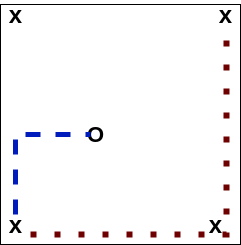
\includegraphics[width=4cm]{text/images/corner.png}
         \caption{O posibila stare initiala}
         \label{fig:corner}
         \end{figure}
    \item ideea consta in faptul ca daca agentul alege sa mearga la cel mai apropiat colt de el, va suporta consecinta de a merge din acel colt la cel mai indepartat colt de coltul respectiv 
    \item liniile 18-21: se extrag colturile nevizitate cand agentul e in starea \textit{state}
    \item liniile 23-24: se rezolva situatia in care starea e scop si atunci euristica trbeuie sa returneze valoarea 0
    \item linia 27: calculare distanta cea mai scurta catre un colt cu manhattan facandu-se abstractie de pereti
    \item linia 31: calculare distanta cea mai lunga catre un colt din coltul determinat la instructiunea precedenta 
    \item 34 : euristica va fi suma dintre aceste doua distante \newline
\end{itemize}


\textbf{Commands:}
\begin{itemize}
    \setlength\itemsep{0em}
    \item -l mediumCorners -p SearchAgent -a fn=aStarSearch,prob=CornersProblem,heuristic=cornersHeuristic
    \item  -l bigCorners -p SearchAgent -a fn=aStarSearch,prob=CornersProblem,heuristic=cornersHeuristic
\end{itemize}

\subsubsection{Questions}

\textbf{Q1:} Test  with  on the mediumMaze layout. What is your number of expanded nodes?

\textbf{A1:} 783 numarul total de noduri expandate, iar costul e de 106


\subsubsection{Personal observations and notes}
% descrieti aici orice fel de probleme ati intampinat in timpul rezolvarii acestui task si modul cum in care le-ati solutionat

% ============================================= Food heuristic ============================= 
\subsection{Question 7 - Eat all food dots - Heuristic definition}
% enuntul intrebarii
In urmatoarele paragrafe va fi prezentata rezolvarea exercitiului 3.5 dib laborator: \newline


\textit{"Propose a heuristic for the problem of eating all the food-dots. The problem of eating all food-dots is already implemented in \textbf{FoodSearchProblem} in searchAgents.py."}.


\subsubsection{Code implementation}
 In continuare se regaseste codul propus pentru implemetarea acestei metode ce descrie o euristica consistenta pentru problema CornersProblem. In incercarea de implementare si apoi testare a solutiei propuse s-au apelat mai multe comenzi din terminal pentru a vedea evolutia agentului pacman in procesul de cautare a solutiei sale \newline \\

\textbf{Code:}

% a se completa fisierul code/6_consisntency_heuristic.py
\inputminted[linenos]{python}{code/07_find_food.py}


\textbf{Explanation:}
\begin{itemize}
    \setlength\itemsep{0em}
    \item ideile prezentate in sectiunea anterioara sun valabile si pentru aceasta subsectiune
    \item ideea este asemnatoare cu cea de la cornerHeuristic
    \item la liniile 5-6: se rezolva cazul in care starea curenta e scop, caz in care euristica trebuie sa fie 0
    \item la linia 10: se calculeaza distanta de la agent pana la cea mai apropiata bucata de mancare, si se determina si pozitia acesteia
    \item la linia 11: se calculeaza distanta de la bucata de mancare determinata anterior pana la cea mai indepartata bucata de mancare fata de aceasta. 
    \item euristica va fi data de suma acestor doua distante
    \item ideea de la care am plecat a fost ca daca agentul alege calea cea mai usoara (adica se indreapta spre cea mai apropiata bucata de mancare), el va suporta consecinta de a merge de la acea bucata de mancare pana la cea mai indeparatata bucata de mancare
\end{itemize}


\textbf{Commands:}
\begin{itemize}
    \setlength\itemsep{0em}
    \item -l testSearch -p SearchAgent -a fn=astar,prob=FoodSearchProblem,heuristic=foodHeuristic
\end{itemize}

\subsubsection{Questions}

\textbf{Q1:} Test  with  autograder \textit{python autograder.py}. Your score depends on the number of expanded states by A* with your heuristic. What is that number?

\textbf{A1:} Numarul de noduri expandate: 8178





% ============================================= SUBOPTIMAL ============================================= 
\subsection{Question 8 - Suboptimal Search}
% enuntul intrebarii
In aceasta sectiune este prezentata o metoda suboptimala:\newline

\textit{"Implement the function findPathToClosestDot in searchAgents.py. Our agent solves this maze (suboptimally!) in under a second with a path cost of 350:"}


\subsubsection{Code implementation}
In continuare se regaseste codul propus pentru implemetarea clasei \textbf{AnyFoodSearchProblem} care decrie o problema ce se poate rezolva suboptimal. In incercarea de implementare si apoi testare a solutiei propuse s-au apelat mai multe comenzi din terminal pentru a vedea evolutia agentului pacman in procesul de cautare a solutiei sale \newline \\


\textbf{Code:}
% a se completa fisierul code/ucs.py
\inputminted[linenos]{python}{code/08_suboptimal.py}

\textbf{Explanation:}
\begin{itemize}
    \setlength\itemsep{0em}
    \item ideea consta in faptul ca agentul mananca de fiecare data cea mai apropiata bucata de mancare, ceea ce ii confera o logica greedy de rezolvare a solutiei
    \item in aceste conditii, metoda \textbf{isGoalState(self, state)} a problemei \textit{AnyFoodSearchProblem} este foarte simpla si se rezuma la verificarea daca starea curenta prezinta o pozitie cu mamncare sau nu. In cazul in care e pozitie cu mancare se va returna True.
    \item in metoda \textbf{findPathToClosestDot}, determinarea actiunilor se va face cu ajutorul parcurgerii bfs pe problema \textit{AnyFoodSearchProblem}, aceasta parcurgere radiala va duce la cea mai scurta cale spre scop

\end{itemize}


\textbf{Commands:}
\begin{itemize}
    \setlength\itemsep{0em}
    \item  -l bigSearch -p ClosestDotSearchAgent -z .5
        
\end{itemize}

\vspace{0.75cm}

\subsection{References}
R. Stuart, N. Peter, Artificial Intelligence: A Modern Approach, 4th US ed., capitol 3, [online] \newline
Curs Inteligenta Artficiala, Universitatea Tehnica din Cluj Napoca, furnizat: moodle.cs.utcluj.ro

% ====================== ADVERSARIAL SEARCH=============================
\section{Adversarial search}

% ============================================= Improve the ReflexAgent ============================= 
\subsection{Question 8 - Improve the ReflexAgent}
% enuntul intrebarii
In aceasta sectiune va fi descris exercitiul 4.8 din laborator: \newline

\textit{"Improve the ReflexAgent such that it selects a better action. Include in the score food locations and ghost locations. The layout testClassic should be solved more often."}.


\subsubsection{Code implementation}
In continuare se regaseste descrirerea perceptiei de moment a agentului. In incercarea de implementare si apoi testare a solutiei propuse s-au apelat mai multe comenzi din terminal pentru a vedea evolutia agentului pacman in procesul de cautare a solutiei sale \newline \\


\textbf{Code:}

% a se completa fisierul code/8_reflex_agent.py
\inputminted[linenos]{python}{code/08_reflex_agent.py}


\textbf{Explanation:}
\begin{itemize}
    \setlength\itemsep{0em}
    \item am aplicat mai multe aporturi pentru perceptia de moment a agentului; in primul rand am luat in calcul cat de aproape se afla de mancare, cat de departe se afla de fantome si cate miscari sunt valabile in momentul in care vor fi inghetate fantomele
    \item distanta fata de mancare trebuie sa contribuie invers proportional la perceptia totala, deoarece cu cat mancarea e mai departe, cu atat nu ii convine agentului situatia. De aceea score-ului final o sa ii adun inversul distantelor fata de mancare. Cu cat distanta e mai mica, cu ata aportul la rezultatul final e mai mare. (linia 11)
    \item cu cat fantomele sunt mai departe, cu atat e mai bine agentului, de aceea o sa adun score-ului a suta parte din distantele fata de fantome (linia 13)
    \item numarul de miscari cand fantomele sunt inghetate va contribui cu a 100 parte la rezultatul final (linia 16)
    

\end{itemize}


\textbf{Commands:}
\begin{itemize}
    \setlength\itemsep{0em}
    \item -p ReflexAgent -l testClassic
    \item  --frameTime 0 -p ReflexAgent -k 1 -l mediumClassic
    \item -p ReflexAgent -l openClassic   
\end{itemize}

\subsubsection{Questions}

\textbf{Q1:} Test your agent on the openClassic layout. Given a number of 10 consecutive tests, how many types did your agent win? What is your average score (points)?

\textbf{A1:} 9/10 meciuri castigate. O medie de aproximativ 1230 de puncte


\subsubsection{Personal observations and notes}
In cele 10 incercari, agentul nu a mancat acea bucata de mancare care ar fi inghetat fantoma

\vspace{0.75cm}

% ============================================= H-Minimax algorithm ============================= 
\subsection{Question 9 - H-Minimax algorithm}
% enuntul intrebarii
Aceasta sectiune este dedicata exercitiului 4.9 din laborator si se cere: \newline

\textit{" Implement H-Minimax algorithm in MinimaxAgentclass from multiAgents.py. Since it can be more  than one ghost, for each max layer there are one ormore min layers."}.


\subsubsection{Code implementation}
In continuare este implementat si explicat algoritmul minimax. In incercarea de implementare si apoi testare a solutiei propuse s-au apelat mai multe comenzi din terminal pentru a vedea evolutia agentului pacman in procesul de cautare a solutiei sale \newline \\

\textbf{Code:}

% a se completa fisierul code/9_h_minimax.py
\inputminted[linenos]{python}{code/09_h_minimax.py}


\textbf{Explanation:}
\begin{itemize}
    \setlength\itemsep{0em}
    \item acest algoritm este de tipul \textbf{adversial search} in care doi sau mai multi agenti au scopuri diferite si se formeaza un mediu competitiv; in cazul jocului pacman avem doua tipuri de agenti: pacman care este agentul MAX si fantomele care sunt agentii MIN. 
    \item algoritmul de fata este insipirat din [1] si a fost adaptat pentru cazul in care sunt mai multi adversari, iar atunci exista mai multe nivele pentru MIN (fantome)
    \item o alta cosntrangere e adancimea pana la care sa se calculeze evaluarea starilor. Din punct de vedere al timpului de executie, este extrem de greu sa se parcurga intreg \textbf{game tree-ul} 
    \item ideea consta in faptul ca valoarea returnata de  \textbf{h\_minimax}  reprezinta utilitatea pentru agentul MAX de a fi in acea stare. MAX prefera o stare cu o valoare maxima, pe cand MIN prefera o stare cu valoare minima
    \item deoarece avem mai multi agenti de tip MIN, atunci trebuie sa se formeze mai multe nivele cu acestia; se considera actiunile fantomelor secvential 
    \item algoritmul propus tine cont si de adancimea maxima la care se va parcurge game tree-ul si este reprezentata de variabila \textbf{depth}
    \item liniile 13-17: este implementata o functie care face testul de cut-off; algoritmul de cautare a unei stari optime se termina in momentul in care starea respectiva duce la pierderea sau castigul jocului sau se afla la adancimea limita pe care am impus-o pentru parcurgerea game tree-ului
    \item functia \textbf{h\_minimax} va fi functia care se va apela de MAX si MIN. In momentul in care agentul este MAX (s-a ajuns la numarul maxim de agenti ai jocului- linia 23), atunci s-a terminat un nivel de cautare si se incrementeaza variabila \textit{depth}. In functie de randul agentului, se va merge pe una dintre cele doua ramuri de la liniile 32-36
    \item metoda \textbf{max\_value} va fi apelata de MAX si ea va returna o actiune nula si evaluarea in starea respectiva daca nu exista alternative de plecare din starea aceea, sau va lua valoarea maxima a stariilor succesoare cu actiunea aferenta
    \item metoda \textbf{min\_value} va fi apelata de MIN si ea va returna o actiune nula si evaluarea in starea respectiva daca nu exista alternative de plecare din starea aceea, sau va lua valoarea minima dintre starile succesoare cu actiunea aferenta
    \item s-a folosit list comprehension
\end{itemize}


\textbf{Commands:}
\begin{itemize}
    \setlength\itemsep{0em}
    \item -p MinimaxAgent -l minimaxClassic -a depth=4
    \item -p MinimaxAgent -l trappedClassic -a depth=3
        
\end{itemize}

\subsubsection{Questions}

\textbf{Q1:} Test Pacman on trappedClassic layout and try to explain its behaviour. Why Pacman rushes to the ghost?

\textbf{A1:} Deoarece sansele lui Pacman de a manca bucatile de mancare sunt foarte mici, el alege varianta de a muri cat mai repede, deoarece functia de evaluare a starilor tine cont si de scorul jocului. Astfel cu cat moare mai repede in asemnea situatie el va castiga mai multe puncte. De aceea se grabeste catre fantoma. Aici joaca un rol important adancimea cu care se apeleaza h\_minimax.


\vspace{0.75cm}

% =============================================  a-b pruning in ABAgent ============================= 
\subsection{Question 10 -  Use $\alpha - \beta$ pruning in AlphaBetaAgent}
% enuntul intrebarii
Aceasta sectiune este dedicata exercitiului 4.11 din laborator si se cere: \newline


\textit{" Use alpha-beta prunning in \textbf{AlphaBetaAgent} from multiagents.py for a more efficient exploration of minimax tree."}.


\subsubsection{Code implementation}
In continuare este implementat si explicat algoritmul minimax cu $\alpha-\beta$ prunning. In incercarea de implementare si apoi testare a solutiei propuse s-au apelat mai multe comenzi din terminal pentru a vedea evolutia agentului pacman in procesul de cautare a solutiei sale \newline \\

\textbf{Code:}

% a se completa fisierul code/10_ab_prunning.py
\inputminted[linenos]{python}{code/10_ab_prunning.py}


\textbf{Explanation:}
\begin{itemize}
    \setlength\itemsep{0em}
    \item acesta algoritm vine pentru a reduce numarul de stari explorate din arborele jocului; 
     \begin{itemize}
        \setlength\itemsep{0em}
        \item$\alpha$ - reprezinta valoarea celei mai bune alegeri dintre punctele de decizie de-a lungul caii pentru MAX, iar 
        \item $\beta$ -reprezinta valoarea cea mai buna (cea mai mica) a unei alegeri pe care o face MIN de-a lungul caii sale decizionale
        \end{itemize}
    \item codul repectiv a fost inspirat din [1] 
    \item prin aceasta tehnica o mare parte din arbore nu va fi explorata daca nu va influenta cu nimic iesirea
    \item terminarea algoritmului este data de aceeasi functie de cut\_off\-test, iar metoda \textbf{h\_alpha\_beta\_prunning} este simimara cu \textbf{h\_minmax} numai ca are doi parametri in plus (alfa si beta)
    \item in cadrul metodei \textbf{max\_value} pe care o va executa agentul MAX, se va lua fiecare stare succesoare si se va calcula evaloarea acetei stari de decizie. Daca valoarea curent obtinua e mai buna decat cea pentru starea anterioara atunci se va actualiza starea in care va merge  agentul, si se va actualiza si valoarea alpha (linia 58) daca valoarea obtinuta este mai buna decat cea pe care am avut-o inainte. Ideea de prunning o regasim la linia 59, unde daca valoarea obtinuta pentru o stare este mai mare decat beta, atunci nu mai are rost sa se continue cu expandarea succesorilor
    \item aceeasi logica este aplicata si pentru \textbf{min\_value} 
    
\end{itemize}


\textbf{Commands:}
\begin{itemize}
    \setlength\itemsep{0em}
    \item  -p AlphaBetaAgent -a depth=3 -l smallClassic

        
\end{itemize}

\subsubsection{Questions}
This sub-section is dedicated to the additional questions that come along with the exercise. Please answer to the following questions:\newline


\textbf{Q1:} Test your implementation with autograder \textbf{python autograder.py} for Question 3. What are your results?

\textbf{A1:} Question q3: 5/5

\subsubsection{Personal observations and notes}
% descrieti aici orice fel de probleme ati intampinat in timpul rezolvarii acestui task si modul cum in care le-ati solutionat

\vspace{0.75cm}

\subsection{References}
[1]R. Stuart, N. Peter, Artificial Intelligence: A Modern Approach, 4th US ed., capitol 3, [online] \newline
[2]Curs Inteligenta Artficiala, Universitatea Tehnica din Cluj Napoca, furnizat: moodle.cs.utcluj.ro

% ====================== PROPRIETARY PROBLEM ===========================
\section{Personal contribution}

% =============================================  a-b pruning in ABAgent ============================= 
\subsection{Question 11 - Define and solve your own problem.}
% enuntul intrebarii
In aceasta sectiune va fi descris un algoritm de cautare pe care l-am propus: \newline

%%%%% PLEASE WRITE THE PROBLEM DEFINITION HERE %%%%%%%
\textit{" Algorimul propus pentru implementare este bidirectional search pe A* , algoritm care in mod simultan face doua cautari: forward -de la starea initiala la scop si backward- de la scop la starea initiala. Speranta acestei abordari consta in coliziunea dintre cele doua cai, si apoi constructia caii finale. Principala motivatie pentru un astfel de algoritm este de a obtine un timp de cautare mai bun, astfel problema se poate imparti in 2, fiecare cu o complexitate de b\textsuperscript{(d/2)}. In consecinta, de la oproblema de complexitate O(b\textsuperscript{d} vom ajunge la o complexitate de O( b\textsuperscript{(d/2)} +  b\textsuperscript{(d/2)}) = O(b\textsuperscript{(d/2)})"}.


\subsubsection{Code implementation}
In aceasta subsectiune se va explica implementarea algoritmului propus si a testelor ce au fost realizate pentru verificarea corectitudinii solutiei propuse. \\

\textbf{Code:}

% a se completa fisierul code/11_prop_problem.py
\inputminted[linenos]{python}{code/11_prop_problem.py}


\textbf{Explanation:}
\begin{itemize}
    \setlength\itemsep{0em}
    \item codul este dupa pseudocodul din [1]
    \item  pentru implementarea acestui algoritm s-a folosit structura de date \textbf{PriorityQueue} din util pentru a delimita frontierele
    \item metoda \textbf{function} va calcula evaluarea unui nod in functie de costul caii din starea initiala la el si o estimare a costului pana la scop. Estimarea se va face printr-o euristica ce va fi ca mod default distanta manhattan
    \item metoda \textbf{bidirectional\_best\_first\_search} va descrie logica de parcurgere a grafului. Pentru structura unui nod s-a folosit aceeasi clasa ca la celelalte solutii propuse anterior (bfs, dfs etc.). 
        \begin{itemize}
        \setlength\itemsep{0em}
        \item la liniile 6 si 10 se vor crea nodurile de start pentru cele dua parcurgeri : forward si backward. Pentru nodul de start al parcurgerii backward se va lua scopul problemei
        \item liniile 10-11: se creeaza o noua problema pentru backward in care se seteaza ca scopul starea initiala a problemei pentru forward
        \item se creeza doua frontiere pentru cele 2 parcurgeri, si aceseat vor fi cozi de prioritati, iar prioritatea este data prin functia \textbf{function}
        \item liniile 20-21: se creeaza doua dictionare de forma stare:nod (stare si nodul asociat ei). care vor fi populate cu nodurile explorate
        \item la linia 23 se initializeaza o solutie care are ca si cost o valoare foarte mare
        \item in bucla de parcuregere a grafului va fi conditionata de existanta de noduri in cele doua frontiere si de conditia de terminare data de metoda  \textbf{terminated}. In cazul in care suma costurilor primelor noduri din cele doua frontiere e mai mare decat ceea ce avem in solutia curenta, atunci nu mai continuam parcurgerea grafului si intoarcem solutia.
        \item linia 33: se evalueaza cele doua noduri fruntase din cele doua frontiere pentru a decide pe care dintre ele sa le expandam (sa le determinam succesorii). Expandarea succesorilor se va face in metoda \textbf{proceed} . Daca starea nodului succesor nu se afla in reached, sau daca pentru aceasta situatie costul de a ajunge in starea asta e mai mic decat costul pe care il aveam deja din alta cale, se va actualiza valoarea la lnia 67 (de aceea am ales implementarea lui \textbf{reached} cu dictionar). Aceasta ultima remarca va duce la gasirea caii optime in toate cazurile pentru acet algoritm.  La linia 70 se va verifica coliziunea dintre parcurgerea forward si backward si in caz afirmativ se va face concatenarea celor doua cai (se tine cont de cadrul in care s-a realizat coliziunea prin \textit{dir}) 
        \end{itemize}
    \item metoda \textbf{join\_nodes} va concatena cele doua cai forward si backward. nf- va fi ultimul nod din calea de forward (calea se obtine prin relatia parinte) si nb - va fi ultimul nod din calea backward. Ideea consta in refacerea legaturilor parinte. Deoarece pentru parcurgerea backward avem cumva oglinda pentru cea forward, trebuie inversata si logica actiunilor (liniile 45-54).
    \item metoda \textbf{a\_star\_bidirectional} va apela \textit{bidirectional\_best\_first\_search} si prin apelul metodei construct\_path (metoda prezentata la dfs) va construi lista de actiuni din relatiile copil parinte 

\end{itemize}


\textbf{Commands:}
\begin{itemize}
    \setlength\itemsep{0em}
    \item  -l tinyMaze -p SearchAgent -a fn=bis
    \item  -l bigMaze -p SearchAgent -a fn=bis -z .5
    \item -l mediumMaze -p SearchAgent -a fn=bis -z .5
        
\end{itemize}
\subsubsection{Personal observations and notes}
Algoritmul este optimal deoarece tot timpul returneaza solutia de cost minim. mediumMaze: 68 costul, 250 noduri expandate; bigMaze: 210 costul, 594 noduri expandate ; tinyMaze: 8 costul, 16 noduri expandate

\vspace{0.75cm}

\vspace{0.75cm}

\subsection{References}
[1]R. Stuart, N. Peter, Artificial Intelligence: A Modern Approach, 4th US ed., capitol 3, [online] \newline
[2] https://notebook.community/aimacode/aima-python/search4e

\end{document}